\documentclass[crop]{standalone}

\usepackage{amsmath}

\usepackage{tikz}

\usetikzlibrary{shapes,decorations,arrows,calc,arrows.meta,fit,positioning}
\tikzset{
    -Latex,auto,node distance =1 cm and 1 cm,semithick,
    O/.style ={rectangle, draw, minimum width = 0.7 cm},
    U/.style ={rectangle, draw, minimum width = 0.7 cm, dashed},
    point/.style = {circle, draw, inner sep=0.04cm,fill,node contents={}},
    bidirected/.style={Latex-Latex,dashed},
    el/.style = {inner sep=2pt, align=left, sloped}
}

\begin{document}

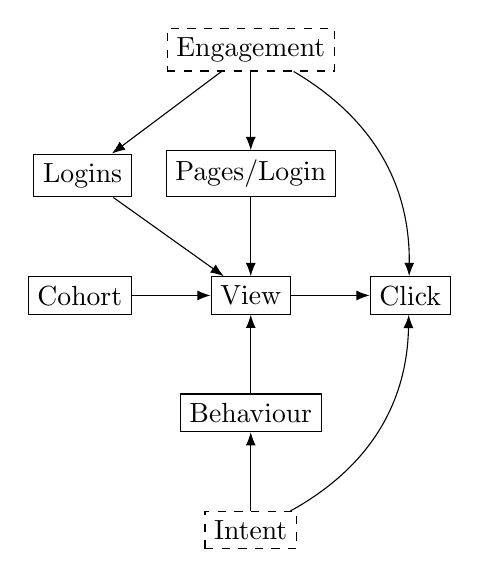
\begin{tikzpicture}
  \node[O] (x) at (0,0) {Cohort};
  \node[O] (m) [right =of x] {View};
  \node[O] (y) [right =of m] {Click};
  \node[O] (m11) [above left =of m] {Logins};
  \node[O] (m12) [above =of m] {Pages/Login};
  \node[U] (c1) [above =of m12] {Engagement};
  \node[O] (m2) [below =of m] {Behaviour};
  \node[U] (c2) [below =of m2] {Intent};
  \path (x) edge (m);
  \path (m) edge (y);

  \path (c1) edge[bend left=30] (y);
  \path (c1) edge (m11);
  \path (c1) edge (m12);

  \path (m11) edge (m);
  \path (m12) edge (m);

  \path (c2) edge[bend right=30] (y);
  \path (c2) edge (m2);
  \path (m2) edge (m);
\end{tikzpicture}

\end{document}
